\documentclass{beamer}
\usepackage[utf8]{inputenc}

\usetheme{Madrid}
\usecolortheme{default}
\usepackage{amsmath,amssymb,amsfonts,amsthm}
\usepackage{txfonts}
\usepackage{tkz-euclide}
\usepackage{listings}
\usepackage{adjustbox}
\usepackage{array}
\usepackage{tabularx}
\usepackage{gvv}
\usepackage{lmodern}
\usepackage{circuitikz}
\usepackage{tikz}
\usepackage{graphicx}

\setbeamertemplate{page number in head/foot}[totalframenumber]

\usepackage{tcolorbox}
\tcbuselibrary{minted,breakable,xparse,skins}



\definecolor{bg}{gray}{0.95}
\DeclareTCBListing{mintedbox}{O{}m!O{}}{%
  breakable=true,
  listing engine=minted,
  listing only,
  minted language=#2,
  minted style=default,
  minted options={%
    linenos,
    gobble=0,
    breaklines=true,
    breakafter=,,
    fontsize=\small,
    numbersep=8pt,
    #1},
  boxsep=0pt,
  left skip=0pt,
  right skip=0pt,
  left=25pt,
  right=0pt,
  top=3pt,
  bottom=3pt,
  arc=5pt,
  leftrule=0pt,
  rightrule=0pt,
  bottomrule=2pt,
  toprule=2pt,
  colback=bg,
  colframe=orange!70,
  enhanced,
  overlay={%
    \begin{tcbclipinterior}
    \fill[orange!20!white] (frame.south west) rectangle ([xshift=20pt]frame.north west);
    \end{tcbclipinterior}},
  #3,
}
\lstset{
    language=C,
    basicstyle=\ttfamily\small,
    keywordstyle=\color{blue},
    stringstyle=\color{orange},
    commentstyle=\color{green!60!black},
    numbers=left,
    numberstyle=\tiny\color{gray},
    breaklines=true,
    showstringspaces=false,
}
%------------------------------------------------------------

\title
{4.12.48}
\author 
{AI25BTECH11034 - Sujal Chauhan }



\begin{document}

\frame{\titlepage}
\begin{frame}{Question}
Prove that if a plane has the intercept a,b,c and is at a distance of p units from the origin, then $\frac{1}{a^2}+\frac{1}{b^2}+\frac{1}{c^2}=\frac{1}{p^2}$

\end{frame}
\begin{frame}{Solution}

\begin{align}
    \begin{tabular}{|c|c|} \hline
    Point   & Positon vector  \\ \hline
     a    & \myvec{a\\ 0 \\0} \\ \hline
     b    & \myvec{0\\ b \\0} \\ \hline
     c    & \myvec{0\\ 0 \\c} \\ \hline
    \end{tabular}
\end{align}
Equation of plane in vector form is given by 
\begin{align}
    \Vec{n}^T\Vec{P}=d
\end{align}
\end{frame}
\begin{frame}{Solution}
where $\Vec{n}$ is normal unit vector to the plane and $d$ is the distance of the plane from the origin. \\
Now given plane satisfys the vectors
\begin{align}
    \myvec{a & 0 & 0 \\
           0 & b & 0 \\
           0 & 0 & c}\Vec{n}=\myvec{p\\ p\\p}
\end{align}

Now multiply both side with inverse of the matrix
\begin{align}
    \Vec{n}=\frac{1}{abc}\myvec{{bc}& 0 & 0 \\
           0 &{ac} & 0 \\
           0 & 0 & {ab}}\myvec{p\\ p\\p}
\end{align}
\begin{align}
    \Vec{n}=\myvec{\frac{p}{a}\\ \frac{p}{b}\\ \frac{p}{c}}
\end{align}
\end{frame}
\begin{frame}{Solution}
Now since $\Vec{n}$ is a unit vector then 
\begin{align}
    \Vec{n}^T\Vec{n}=1
\end{align}
\begin{align}
    \frac{1}{a^2}+\frac{1}{b^2}+\frac{1}{c^2}=\frac{1}{p^2}
\end{align}
    
\end{frame}
\begin{frame}{Figure}
    \begin{figure}
        \centering
        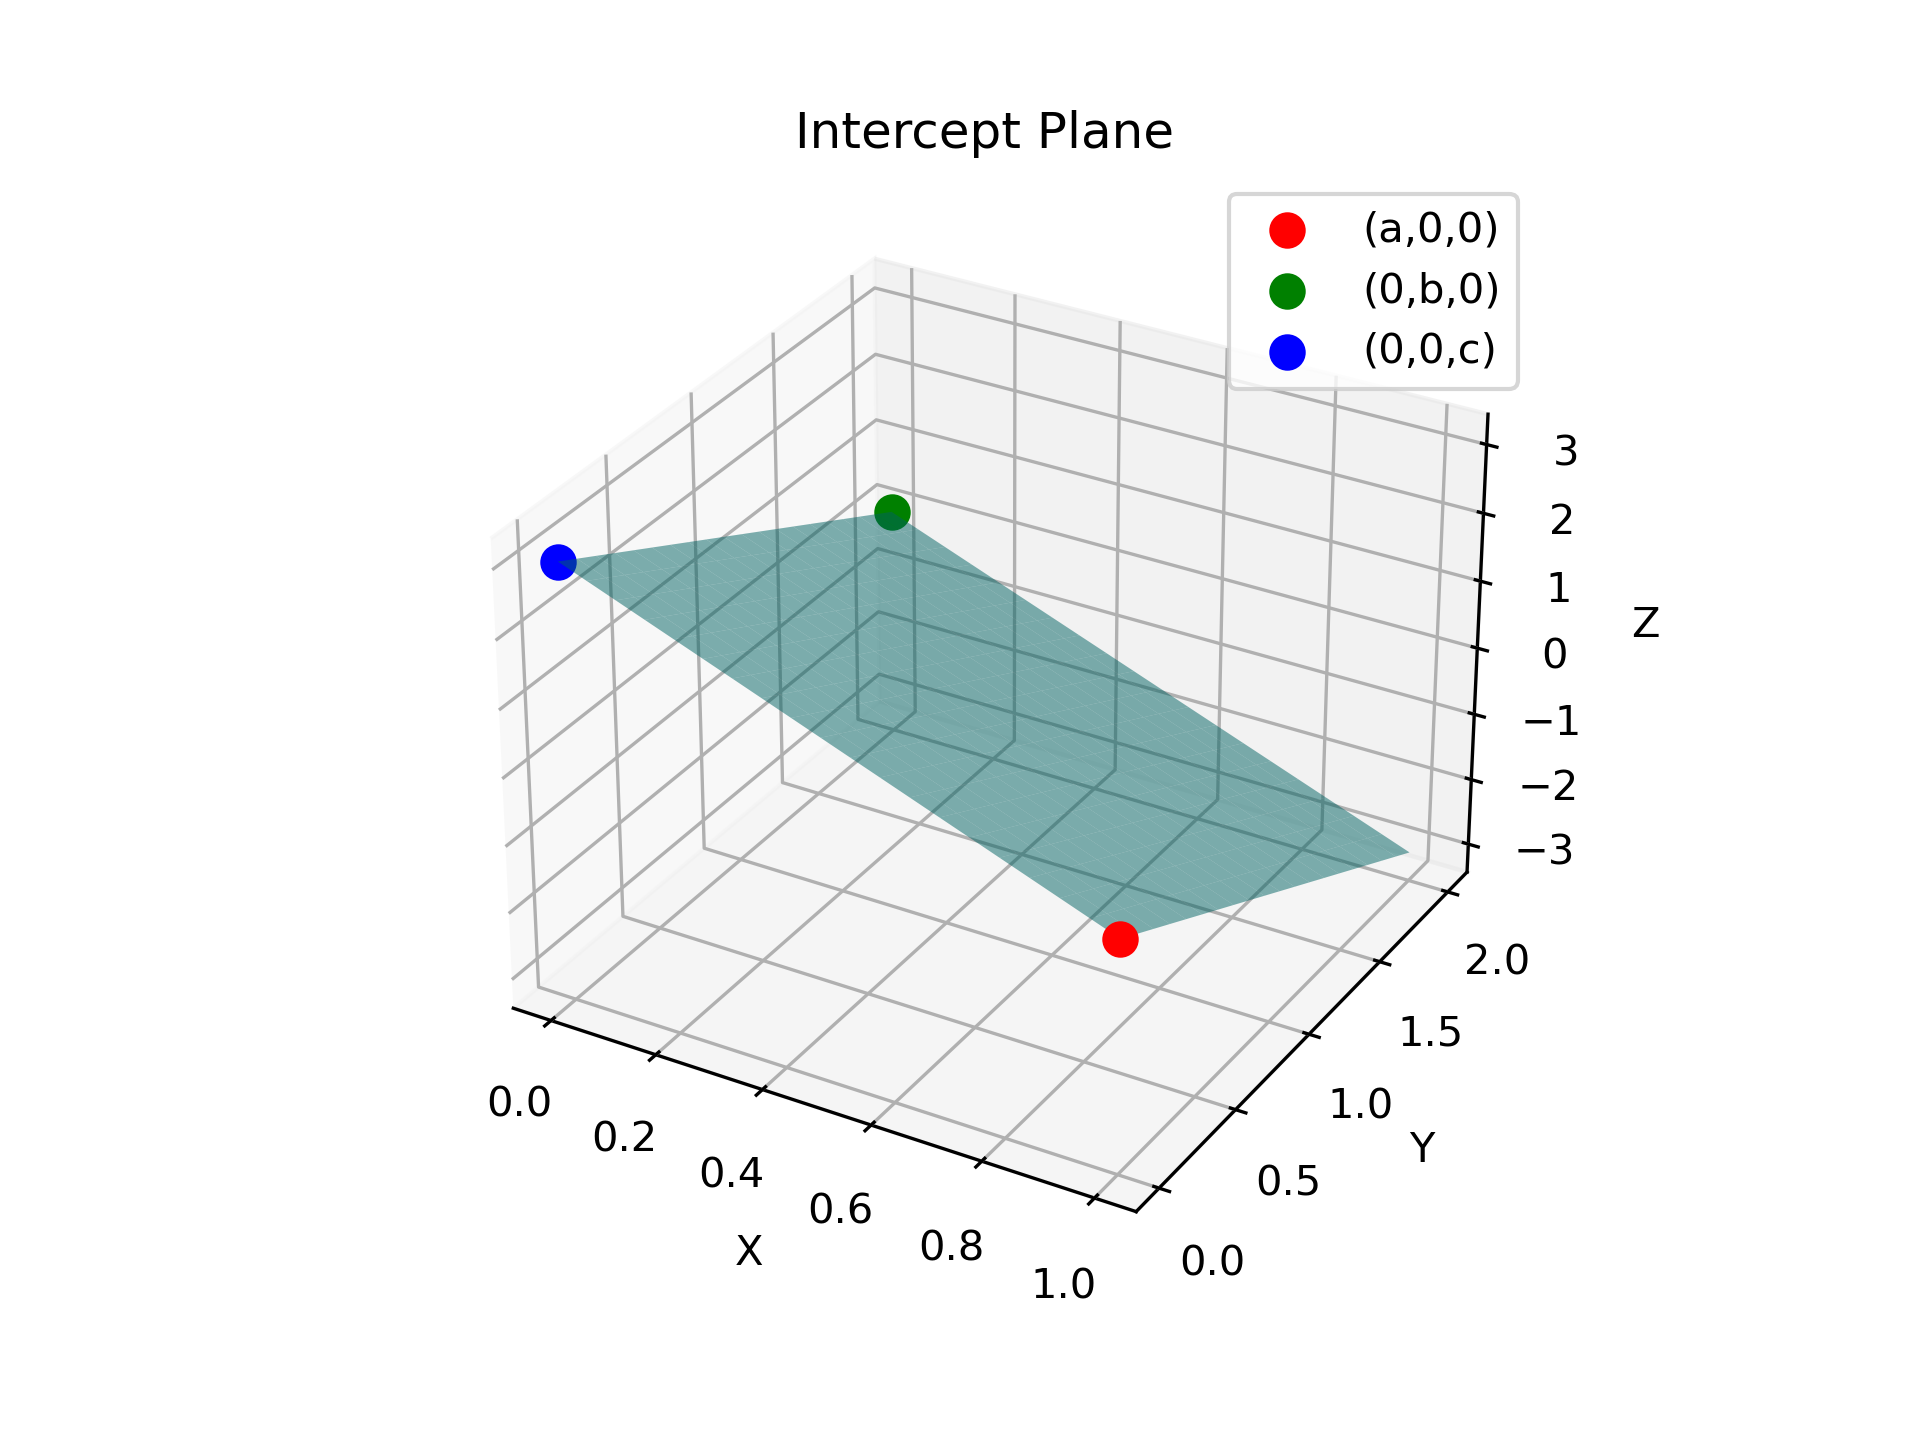
\includegraphics[width=0.5\linewidth]{figures/intercept_plane.png}
        \caption{Ploting}
        \label{fig:placeholder}
    \end{figure}
\end{frame}
\end{document}
